% !TEX encoding = UTF-8
% !TEX TS-program = pdflatex
% !TEX spellcheck = it-IT
%% !TEX root = 
%% !BIB TS-program = biber

\documentclass[
	12pt,
	%German, % Uncomment for German
]{sty/report_style}
% \documentclass{article}
\usepackage[final, nonatbib]{sty/nips_2018}
\usepackage{sty/article_defaults}
\newcommand{\todo}[1]{\textcolor{red}{TODO: #1}}

\setminted[python]{linenos, breaklines, fontsize=\footnotesize}

%-------------------------------------------------------
%	ASSIGNMENT INFORMATION
%-------------------------------------------------------

\title{Practical Course on Computer Vision and Robotics} % Assignment title

\authorOne{Tommaso Bertola, 25544550} % Student name
\authorTwo{Marco Martinico, 27144566} % Student name
\authorThree{Roberto Togni, 23340265} % Student name

\date{15.02.2024} % Due date

\institute{Georg-August-Universität Göttingen \\ Drittes Physikalisches Institut} % Institute or school name

\class{Practical Course on Computer Vision \& Robotics} % Course or class name

\professor{Sebastian Ruiz, Lennart Jahn} % Professor or teacher in charge of the assignment

%-------------------------------------------------------

\begin{document}

\maketitle

%-------------------------------------------------------
%	ASSIGNMENT CONTENT
%-------------------------------------------------------
\begin{problem}
    Write 3-6 pages (excluding appendix) for the following sections. Complete the table in \cref{appendix:time_schedule} and attach interesting pieces of code in \cref{appendix:code}.
\end{problem}

\section{Summary}

%Give a short summary on the methods used and on the major discussion points.

The project involves the construction of a two-wheeled robot using Raspberry Pi for computations and Lego Mindstorms for sensor and movement control. The robot employs reactive control to explore a track, utilizing an application of Extended Kalman Filter (EKF) to the Simultaneous Localization And Mapping (SLAM) algorithm to create an accurate map of the track. Subsequently, the A* algorithm is applied to compute the optimal path, which the robot then follows. To ensure precision in path following, a PID controller has been implemented, thus preventing the robot from deviating from the calculated path.

Throughout the project implementation, we faced various challenges, particularly in the following areas:
\begin{itemize}
    \item Managing the transition between different reference systems;
    \item Developing a robust algorithm for reactive control;
    \item Implementing the EKF\_SLAM algorithm;
    \item Processing the map effectively for use in the A* algorithm.
\end{itemize}

\section{Method}

%Write down your method for solving the task. What was your strategy? How did you construct the robot to perform the task?

%For example, split into sections like this (or however you like):

\subsection{Computer Vision}

The computer vision task was quite complex, as it involved several aspects. For simplicity, we separated it into several tasks. The code used for detecting discs is detailed in \cref{appendix:vision}.

\subsubsection{ArUco markers detection}

To detect the ArUco markers, we used the functions provided by OpenCV. In particular, we used the \verb|estimatePoseSingleMarkers()| method to obtain the traslation and rotation vectors (\verb|tvecs| and \verb|rvecs|, respectively). We then used the values obtained to construct the transformation matrix from the camera to the markers. To obtain the marker positions relative to the robot, we concatenated (i.e. computed the dot product) the transform matrices as shown in \cref{eq:1}:

\begin{equation} \label{eq:1}
T_{\text{robot,marker}} = T_{\text{robot,camera}} \cdot T_{\text{camera,marker}}
\end{equation}

\subsubsection{Discs detection}

To identify red and green discs, we concatenated several image processing techniques within the \verb|find_centroids()| method. First, the input image is converted into the HSV colour space. A colour mask and bitwise operations are then used to identify the red or green areas of the image (we used a range to account for possible artifacts due to illumination and distance from the discs).

We then converted the resulting image to grayscale, applied Gaussian blur, and used a threshold to create a binary image. Morphological operations (opening and closing) are then applied to refine the binary image. The final step utilises connected components analysis to label distinct regions and computes centroids for each labelled component. The function returns the number of labelled components, centroids (x, y coordinates), and statistics about each labelled region. 


Since the coordinates are with respect to the two-dimensional image, the \verb|detect_circle()| function utilises the \verb|img_to_world()| function for transforming image points into corresponding 3D world coordinates.


\subsection{Exploration - Reactive Driving}

The exploration task entails the robot traversing the path twice, with the inner side followed in the first round and the outer side in the second. This sequential approach contributes to the production of a relatively accurate map by the Extended Kalman Filter (EKF) Simultaneous Localization and Mapping (SLAM) algorithm.

The algorithm we used to follow either side is detailed in \cref{appendix:reactctrl}. The underlying logic is straightforward. A variable is employed to determine whether the robot should follow the inner or outer side. Based on this determination, the landmark IDs are filtered to exclusively consider either the outer or inner landmarks. If there are at least two filtered landmarks, the robot adjusts its speed and computes the relative position of these landmarks. The latter is utilized to determine the angle (\verb|theta|) between the two landmarks. The robot then sets the \verb|turn| parameter to control its steering. Since the relationship between angle and \verb|turn| is not linear, some conditional statements are used to set the \verb|turn| value. Additional checks are performed to ensure that the distance to the nearest ArUco markers falls within a specified range. This step proved particularly helpful during the early stages of the task.

If the robot fails to detect at least two ArUco markers, a warning message is printed, and the robot starts rotating in the direction of the side being followed. The speed at this stage is reduced slightly to facilitate ArUco recognition.


\subsection{Mapping}

Since A* takes as input a graph and two points (start and end), we had to process the map obtained by SLAM. In order to do this, we decided to represent the map by means of a matrix, in effect discretizing the environment. The code used to switch between matrix and real-world coordinates is listed in \cref{appendix:map}.

First, we separated outer track, inner track, obstacles and starting line into several arrays. We then processed these to join the individual points by means of a polygon. At this point we switched from real coordinates to indices in the array, maintaining a resolution of 5 cm.

%\todo{Describe ordinator + insert code}

We then used the previously obtained polygons to create a binary mask representing the map. Specifically, we assigned a value of 1 to all non-steppable regions (i.e., outside the outer edge and inside the inner edge), and a value of 0 to all steppable regions (i.e., the track). We also performed a dilation on the inner region in order to prevent the pathfinding algorithm from returning a path excessively close to the inner edge.

Finally, we added the starting line and obstacles to the binary mask, assigning a value of 1 to both. The addition of the starting line proved particularly effective in the context of the pathfinding algorithm, effectively making the choice of heuristics much more trivial.


\subsection{Pathfinding}

The map obtained during exploration is processed in order to use it as input for the A* algorithm (see \cref{appendix:astar}). We opted for this approach for several reasons. First of all, A* guarantees finding the shortest path (if one exists). Secondly, it is more efficient than Dijkstra's algorithm thanks to the heuristic component. 

Since A* requires a starting and an ending point, we had to figure out how to obtain them. To do so, we adopted the following approach: We started by finding the extremes of the start line in the grid; we then converted them to real-world coordinates and computed two circumferences centered in the two points and with a radius equal to three quarters of the distance between them; finally, we found the two points of intersection of the two circumferences and used them as starting and ending points.

\subsection{Path Following}

After obtaining the optimal path via A*, we implemented the logic to follow it. Due to motor uncertainty and wheel slippage, a blind following approach is not feasible. We therefore implemented a PID controller in order to correct the movement in real time and ensure that the robot follows the planned path.

The main problem we encountered in this context turned out to be the execution time of the code. Since the latter is often around 0.5 seconds, the PID correction suffers from an inherent delay, which results in poor performance. To mitigate this problem, we have rewritten several parts of the code in order to reduce latencies as much as possible. This resulted in improved driving, which allowed us to better fine-tune the PID controller.

For the fine-tuning procedure, we followed the following approach. We set all constants to 0, then increased $K_p$ until we observed oscillations in the output. At this point we halved the value of $K_p$ and increased that of $K_i$ until we observed overshoot. We then started increasing $K_d$. At the end of the procedure, we set the values of the three constants to 32, 2 and 0 respectively.

\subsection{Optimisation}\label{sec:optimisation}

Much of the optimisation was focused on reducing code execution times (see \cref{fig:exec_times_exploration} and \cref{fig:exec_times_race}). In particular, we tried to speed up the matrix products performed in the context of the EKF\_SLAM. To do this, we rewrote some functions using the just-in-time compilation service offered by numba. Given the incomplete support for numpy and the conflicts due to the use of OOP, we had to carry out considerable refactoring of the code. However, this approach proved effective, reducing latencies and allowing us to optimise the path-following task.

\section{Results}

%Can you quantify any parts of your method? What is your accuracy in SLAM for example? How well does your path finding perform? etc...

Our robot showed good results in the context of reactive control with respect to the outer side of the track. The discretized map, with a grid element size of 5 cm, provided a reliable basis for the A* pathfinding algorithm to calculate the optimal route.

However, during the exploration phase on the inner side of the track, the robot exhibited difficulties in handling tight bends. This issue likely arose from the limitations of our reactive control approach, which may not have been sufficiently robust for the rapid changes in curvature and direction required in these sections.



\section{Discussion}

%Discuss problems that you encountered with the robot and how you solved them. What worked well? What didn't work so well? What would you improve next time? 

One of the main problems we encountered was the execution time of the code, which introduced a substantial delay in the execution of the various tasks (see \cref{appendix:figures} for an overview of the execution times). One of the parts most affected by this problem is the EKF SLAM, whose execution time becomes problematic as the number of landmarks increases. To try to mitigate this problem, we decided to perform the SLAM:
\begin{itemize}
    \item On two-thirds of the landmarks seen during exploration (\verb|fastmode| not active)
    \item On the (at most) 3 closest bowls during the run (\verb|fastmode| active)
\end{itemize}

Since this did not prove sufficient, we used numba to boost performance for computationally heavy sections as described in \cref{sec:optimisation}.

A second problem we faced was the ordering of the ArUcos, necessary to perform the  transition between a continuous representation of the environment and a discretized one. In particular, we had to develop a mechanism to order the mapped ArUcos so that they could be used as vertices to draw a polygon. The solution we came up with is conceptually simple: the ArUcos are ordered by considering the nearest marker as next, disregarding any ArUcos that are further away than a threshold. This last detail proved to be of critical importance, partially plugging mapping errors. The algorithm is detailed in \cref{appendix:ordinator}.


\section{Teamwork}

Given the complexity of the task, we decided to tackle every aspect together. We opted for this approach for two reasons:
\begin{itemize}
    \item Neither of us had ever worked on such a project. As a consequence, we had to work together to find solutions for the problems we had to face;
    \item Given the complexity of the code, implementing tasks separately would have reduced the awareness each of us had on which section of code did what. This would have resulted in less uniform code as well as taken more time for us to integrate different sections.
\end{itemize}

However, within the individual working sessions we often divided the tasks, so as to speed up the work and come up with more efficient solutions. This approach worked quite well, allowing us to constantly confront different ideas and work on our teamwork skills. The table in \cref{appendix:time_schedule} shows the project timestamps.

%\todo{downside}
%The main downside was

%Discuss how you divided the task. Mention what went well in the division of work and what could have gone better. Fill in the table in \cref{appendix:time_schedule}.

\clearpage
\appendix

\section{Figures}\label{appendix:figures}

\begin{figure}[h]
    \centering
    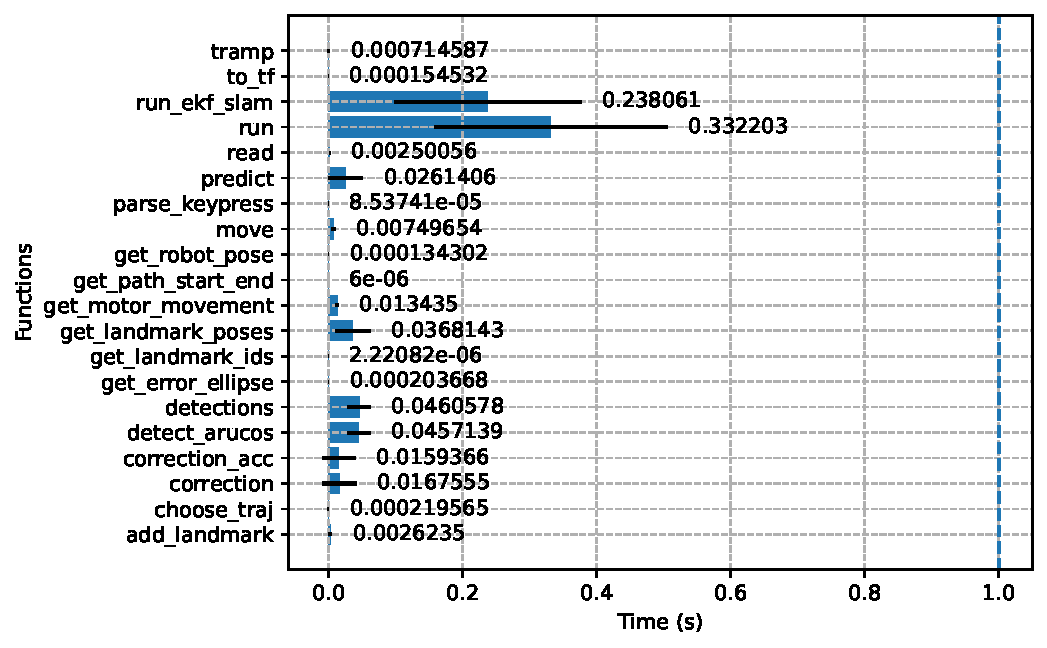
\includegraphics[width=\textwidth]{img/Exploration.pdf}
    \caption{Execution times of the main functions during the exploration rounds.} 
    \label{fig:exec_times_exploration} 
\end{figure}

\begin{figure}[h]
    \centering
    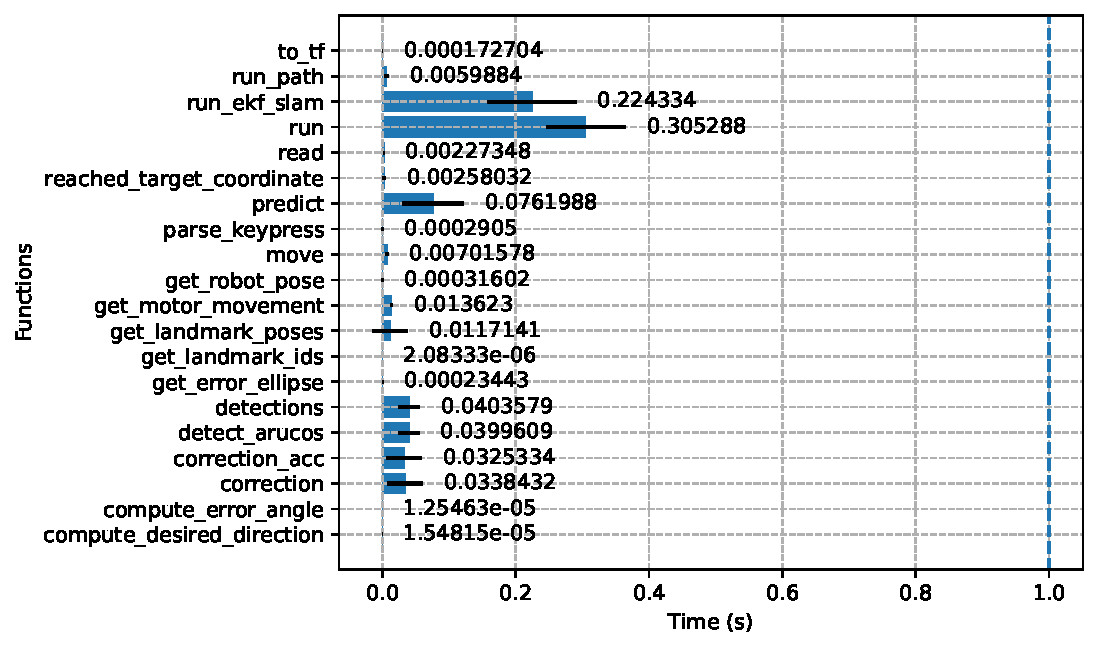
\includegraphics[width=\textwidth]{img/Race.pdf}
    \caption{Execution times of the main functions during the race.} 
    \label{fig:exec_times_race} 
\end{figure}

\newpage
\section{Time Schedule}\label{appendix:time_schedule}

Approximate time schedule and task distribution.

\begin{table}[h]
\begin{tabularx}{\linewidth}{@{}p{2cm}X@{}}%{@{}p{2cm}p{4cm}Xc>{\centering\arraybackslash}c@{}}
\toprule
Date        & Description of Work \\
\midrule
10/11/2023 &   Compiled the OS for the robot and wrote some code to test the motor functions. \\
\addlinespace[0.5em]
10/11/2023 &   Modified config file for robot. \\

\addlinespace[0.5em]
30/11/2023 &   Implemented ArUco and circles detection. Also converted ids to integers and use proper numbering for circles. \\

\addlinespace[0.5em]
03/12/2023 &    Added robot parameters to config. Returned landmark positions with respect to world coordinates. Tested ev3 library.\\

\addlinespace[0.5em]
07/12/2023 &    Wrote EKF prediction step. Improved vision by drawing rectangles around detected ArUcos and cirles.\\

\addlinespace[0.5em]
10/12/2023 &   Fixed some bugs, added possibility to save screenshots from camera. Started implementing correction step in EKFSLAM and made first test with reactive control drive.\\

\addlinespace[0.5em]
14/12/2023 &   Improved reactive control drive.\\


\addlinespace[0.5em]
17/12/2023 &   Modified reactive control to follow outer track, added some correction maneuvres. Added parameters to allow driving in both directions.\\

\addlinespace[0.5em]
21/12/2023 &   Bugfix for dimension of recognized outer ArUco. Started working on inner ArUco recognition.\\

\addlinespace[0.5em]
23/12/2023 &   Improved EKF SLAM.\\

\addlinespace[0.5em]
29/12/2023 &   Worked on EKF SLAM.\\

\addlinespace[0.5em]
10/01/2024 &   Added error ellipses to EKF SLAM.\\

\addlinespace[0.5em]
14/01/2024 &   Fixed EKF SLAM, fixed major error in coordinate system with ArUco detection.\\

\addlinespace[0.5em]
16/01/2024 &   Started working on A*.\\

\addlinespace[0.5em]
17/01/2024 &   Implemented map saving for A* and corrected exploration. Started working on polygon creation from landmark positions.\\

\addlinespace[0.5em]
19/01/2024 &   Finished map conversion for A*.\\

\addlinespace[0.5em]
21/01/2024 &   Implemented A* with temporary function.\\

\addlinespace[0.5em]
24/01/2024 &   Improved reactive control on inner track. Worked on heuristic function for A*. Major speed improvements on EKFSLAM.\\

\addlinespace[0.5em]
25/01/2024 &   Experimented with checkpoints to improve EKF SLAM.\\

\addlinespace[0.5em]
28/01/2024 &   Added load map functionality and added start line and obstacles to the map.\\

\addlinespace[0.5em]
31/01/2024 &   Worked on map conversion between grid and real world. Implemented switch to different tasks and fast mode for EKFSLAM.\\

\addlinespace[0.5em]
04/02/2024 &   Minor corrections on code, started implementing PID for path following. Execution time benchmarking.\\

\addlinespace[0.5em]
07/02/2024 &   Started fine-tuning PID, improved A*.\\

\addlinespace[0.5em]
09/02/2024 &   Created notebook for disc recognition demo.\\

\addlinespace[0.5em]
10/02/2024 &   Optimised code execution time, improved PID controller.\\

\addlinespace[0.5em]
11/02/2024 & Rewrote functions using numba, refactored code moving global variables to config file.\\
\bottomrule
\end{tabularx}
\end{table}


\clearpage
\section{Code}\label{appendix:code}

%Put interesting pieces of code here. Please also send all your code in a .zip file by email to \\ \href{mailto:sebastian.ruiz@uni-goettingen.de}{sebastian.ruiz@uni-goettingen.de}. 

\subsection*{Reactive Control}\label{appendix:reactctrl}

\inputminted{python}{py_files/reactive_control.py}

\subsection*{Computer Vision}\label{appendix:vision}

\inputminted{python}{py_files/vision.py}

\subsection*{Conversion Between Discretized and Real World Coordinates}\label{appendix:map}
\inputminted{python}{py_files/mazerunner.py}

\subsection*{ArUco Markers Rearrangement}\label{appendix:ordinator}
\inputminted{python}{py_files/ordinator.py}

\subsection*{Path Finding Algorithm}\label{appendix:astar}

\inputminted{python}{py_files/astar.py}

%\subsection*{PID Controller}
%\inputminted{python}{example.py}

%\todo{decide whether to include it or not}

\end{document}
